\documentclass[spanish]{extbook}
\usepackage[T1]{fontenc}
\usepackage[utf8]{luainputenc}
\usepackage[a4paper]{geometry}
\usepackage{color}
\usepackage{amsmath}
\usepackage{graphicx}
\usepackage{babel}
\usepackage{listings}
\geometry{verbose}
\makeatletter
\numberwithin{equation}{section}
\numberwithin{figure}{section}
\makeatother
\addto\shorthandsspanish{\spanishdeactivate{~<>}}
\renewcommand{\lstlistingname}{Listado de código}
\title{Introducción a las estadísticas con R}
\date{2018-01-20}
\author{Peter Daalgard}

\begin{document}

\tableofcontents
\newpage

%%%%%%%%%%%%%%%%%%%%%%%%%%%%%%%%%%%%%%%%%%%%%%%%%%%%%%%%%%%%%%%%%%%%%%%%%%%%%%%
%% Prefacio
%%%%%%%%%%%%%%%%%%%%%%%%%%%%%%%%%%%%%%%%%%%%%%%%%%%%%%%%%%%%%%%%%%%%%%%%%%%%%%%
\chapter*{Prefacio}

\textbf{R} es un programa informático de estadístas disponible a través de
Internet bajo la Licencia Pública General (GPL). Es decir, se suministra con
una licencia que le permite utilizarlo libremente, distribuirlo o incluso
venderlo, siempre que el receptor tenga los mismos derechos y el código fuente
esté disponible libremente. Existen versiones para Microsoft Windows XP o
posterior, para una variedad de plataformas Unix y Linux, y para Apple
Macintosh OS X. 

\textbf{R} proporciona un entorno en el que puede realizar análisis
estadísticos y producir gráficos.  En realidad es un lenguaje de programación
completo, aunque eso, en este libro sólo se describe marginalmente. Aquí nos
conformamos con aprender los conceptos elementales y ver varios ejemplos. 

\textbf{R} está diseñado de tal manera que siempre es posible realizar más
cálculos sobre los resultados de un procedimiento estadístico. Además, la
funcionalidad para la presentación gráfica de los datos permite tanto métodos
simples, como por ejemplo \texttt{plot(x, y)}, como también la posibilidad de
un control mucho más fino del aspecto de las gráficas. 

El hecho que \textbf{R} esté basado en un lenguaje formal de computadora le da
una tremenda flexibilidad.  Otros sistemas presentan interfaces más sencillas
en términos de menús y formularios, pero a menudo la aparente facilidad de uso
se convierte en un obstáculo a largo plazo. Aunque las estadísticas elementales
se presentan a menudo como una colección de procedimientos fijos, el análisis
de datos moderadamente complejos requiere la creación de modelos estadísticos
ad-hoc, lo que hace que la flexibilidad añadida de \textbf{R} sea altamente
deseable.

\textbf{R} debe su nombre a una típica humorada de Internet. Es posible que
haya oido hablar del lenguaje de programación C (cuyo nombre es otra historia
en sí misma). Inspirados por esto, Becker y Chambers eligieron, a principios de
los años ochenta, llamar a su nuevo lenguaje de programación estadística S.
Este lenguaje se desarrolló aún más en el producto comercial S-PLUS, que a
finales de la década era de uso generalizado entre los estadísticos de todo
tipo. Ross Ihaka y Robert Gentleman de la Universidad de Auckland, Nueva
Zelanda, eligieron escribir una versión reducida de S para propósitos de
enseñanza, y ¿qué era más natural que elegir la letra inmediatamente anterior?
Las iniciales de Ross y Robert también pueden haber jugado un papel importante. 

En 1995, Martin Maechler persuadió a Ross y Robert para que publicaran el
código fuente de \textbf{R} bajo la licencia GPL. Esto coincidió con el auge
del software de código abierto impulsado por el sistema Linux. R pronto logró
llenar un hueco de gente como yo que tenía la intención de usar Linux para
computación estadística, pero no tenía ningún paquete estadístico disponible en
ese momento. Se creó una lista de correo para la comunicación de informes de
fallos y discusiones sobre el desarrollo de \textbf{R}.

En agosto de 1997, me invitaron a unirme a un equipo internacional extendido
cuyos miembros colaboran a través de Internet y que ha controlado el desarrollo
de \textbf{R} desde entonces. Posteriormente, el equipo básico se amplió varias
veces y actualmente cuenta con 19 miembros. El 29 de febrero de 2000, se
publicó la versión 1.0.0.0. Al momento de estos escritos, la versión actual es
la 2.6.2. Este libro se basó originalmente en una serie de notas elaboradas
para el curso de Estadística Básica para Investigadores en Salud de la Facultad
de Ciencias de la Salud de la Universidad de Copenhague. El curso tenía como
objetivo principal los estudiantes de doctorado en medicina. Sin embargo, el
material se ha revisado sustancialmente y espero que sea útil para un público
más amplio, aunque sigue habiendo algunos sesgos bioestadísticos, especialmente
en la elección de ejemplos. En los últimos años, el curso de Práctica
Estadística en Epidemiología, que se ha celebrado anualmente en Tartu
(Estonia), ha sido una fuente importante de inspiración y experiencia en la
introducción de jóvenes estadísticos y epidemiólogos a \textbf{R}.  Este libro
no es un manual para \textbf{R}.  La idea es introducir una serie de conceptos
y técnicas básicas que deberían permitir al lector comenzar con estadísticas
prácticas. En cuanto a los métodos prácticos, el libro cubre una currícula
razonable para los estudiantes de primer año de estadística teórica, así como
para los estudiantes de ingeniería. Estos grupos eventualmente necesitarán ir
más allá y estudiar modelos más complejos, así como técnicas generales que
involucren programación real en el lenguaje \textbf{R}.

Para los áreas en las que las estadísticas elementales se enseñan
principalmente como una herramienta, el libro va un poco más allá de lo que se
enseña comúnmente a nivel universitario. Los métodos de regresión múltiple o el
análisis de experimentos multifactoriales rara vez se enseñan a ese nivel, pero
pueden convertirse rápidamente en esenciales para la investigación práctica. He
recopilado los métodos más simples al principio para hacer el libro más legible
también en un nivel elemental. Sin embargo, para mantener el material técnico
consistente, los capítulos 1 y 2 sí incluyen material que algunos lectores
querrán omitir. Por lo tanto, el libro pretende ser útil para varios grupos,
pero no pretenderé que pueda valerse por sí solo para ninguno de ellos. He
incluido breves secciones teóricas en relación con los diversos métodos, pero
más que como material didáctico, éstos deberían servir de recordatorios o
quizás como aperitivos para los lectores que son nuevos en el mundo de la
estadística.

%%%%%%%%%%%%%%%%%%%%%%%%%%%%%%%%%%%%%%%%%%%%%%%%%%%%%%%%%%%%%%%%%%%%%%%%%%%%%%%
%% Conceptos Básicos
%%%%%%%%%%%%%%%%%%%%%%%%%%%%%%%%%%%%%%%%%%%%%%%%%%%%%%%%%%%%%%%%%%%%%%%%%%%%%%%
\chapter{Conceptos Básicos}

El propósito de este capítulo es que empiece a usar  \textbf{R}.  Asumimos que
ya tiene una instalación funcional del software y del paquete \texttt{ISwR} que
contiene los conjuntos de datos para este libro. Las instrucciones para obtener
e instalar el software se encuentran en el \index{Apéndice A}. Como ya
mencionamos, el libro describe la versión 2.6.2 de  \textbf{R}.  En la medida
de lo posible, presento los temas de una manera que es independiente del
sistema operativo en uso y asumo que el lector tiene el conocimiento operativo
elemental para seleccionar desde menús, mover ventanas, etc. Sin embargo, hago
excepciones cuando soy consciente de dificultades específicas con una
plataforma o características específicas de la misma.

%%%%%%%%%%%%%%%%%%%%%%%%%%%%%%%%%%%%%%%%%%%%%%%%%%%%%%%%%%%%%%%%%%%%%%%%%%%%%%%
%% Primeros pasos
%%%%%%%%%%%%%%%%%%%%%%%%%%%%%%%%%%%%%%%%%%%%%%%%%%%%%%%%%%%%%%%%%%%%%%%%%%%%%%%
\section{Primeros pasos}

Esta sección ofrece una introducción al entorno informático de  \textbf{R}
Computing y le muestra sus características más básicas. Iniciar  \textbf{R} es
sencillo, pero el método dependerá de su plataforma informática.  Podrá
iniciarlo desde el menú del sistema, haciendo doble clic en un icono o
introduciendo el comando \textquotedbl{}R\textquotedbl{} en la línea de
comandos del sistema. Esto producirá una ventana de consola o hará que
\textbf{R} se inicie como un programa interactivo en la ventana del terminal
actual. 

\begin{figure}[h!]
  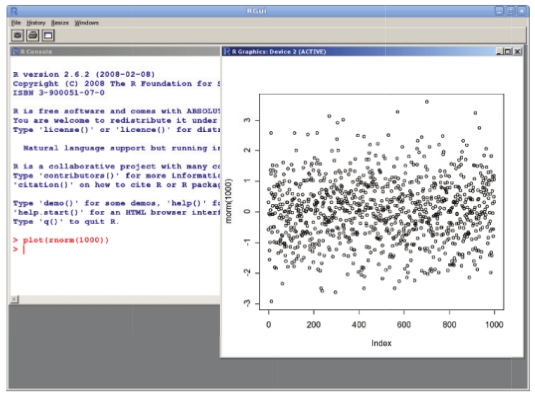
\includegraphics[width=\linewidth]{rwin.png}
  \caption{A boat.}
  \label{fig:rwin}
\end{figure}

Figura \ref{fig:rwin} Captura de patalla de R Windows.

En cualquier caso, R funciona fundamentalmente según el modelo de
preguntas y respuestas:

Ingrese una línea con un comando y pulse \texttt{<ENTER>} (\texttt{<--}).
Entonces el programa hace algo, imprime el resultado si es relevante y pide más
información.

Cuando \textbf{R} está listo para la entrada, imprime su símbolo, un
\textquotedbl{}>\textquotedbl{}.  Es posible usar \textbf{R} como una
aplicación en modo sólo texto, y también en el modo por lotes, pero para los
propósitos de este capítulo, asumo que usted está sentado en una estación de
trabajo gráfica.

Todos los ejemplos de este libro deberían ejecutarse si los escribes
exactamente como están impresos, siempre y cuando tengas el paquete
\texttt{ISwR} no sólo instalado sino también cargado en tu ruta de búsqueda
actual. Esto se hace introduciendo:

\begin{lstlisting}[language=R]
> library(ISwR)
\end{lstlisting}

en la línea de comandos. No necesita entender lo que hace este comando en este
precisomomento. Se explicará en la Sección 2.1.5. Para una primera impresión de
lo que \textbf{R} puede hacer, intente escribir lo siguiente:

\begin{lstlisting}[language=R]
> plot(rnorm(1000))
\end{lstlisting}

Este comando dibuja 1000 números al azar a partir de la distribución normal
(rnorm = \emph{r}andom \emph{norm}al) y los dibuja en una ventana emergente de
gráficos. El resultado en una máquina Windows se puede ver en la Figura 1.1.
Por supuesto, en este momento no esperamos que adivine que obtendría este
resultado de esa forma en particular. Elegimos este ejemplo porque muestra
varios componentes de la interfaz de usuario en acción. Antes de que el estilo
de comandos sea natural para usted, es necesario introducir algunos conceptos y
convenciones a través de ejemplos más simples. Bajo Windows, la ventana de
gráficos tomará el enfoque del teclado en este punto. Haga clic en la consola
para que acepte más comandos.

%%%%%%%%%%%%%%%%%%%%%%%%%%%%%%%%%%%%%%%%%%%%%%%%%%%%%%%%%%%%%%%%%%%%%%%%%%%%%%%
%% Una calculadora gigante
%%%%%%%%%%%%%%%%%%%%%%%%%%%%%%%%%%%%%%%%%%%%%%%%%%%%%%%%%%%%%%%%%%%%%%%%%%%%%%%
\subsection{Una calculadora gigante}

Una de las tareas más simples posibles de hacer en \textbf{R} es introducir una
expresión aritmética y obtener un resultado. (La segunda línea es la respuesta
de la máquina.)

\begin{lstlisting}[language=R]
> 2 + 2 
[1] 4
\end{lstlisting}

De esta forma vemos que la máquina sabe que 2 más 2 son 4. Por supuesto,
también sabe hacer otros cálculos estándar, como ser $e^{-2}$:

\begin{lstlisting}[language=R]
> exp(-2) 
[1] 0.1353353
\end{lstlisting}

El \texttt{{[}1{]}} delante del resultado es parte de la forma en
que \textbf{R} imprime números
y vectores. No es útil aquí, pero lo es cuando el resultado es un
vector más largo. El número entre corchetes es el índice del primer
número de esa línea. Considere el caso de generar 15 números aleatorios
a partir de una distribución normal:

\begin{lstlisting}[language=R]
> rnorm(15) 
[1]  -0.18326112 -0.59753287 -0.67017905 0.16075723  1.28199575
[6]   0.07976977  0.13683303  0.77155246 0.85986694 -1.01506772
[11] -0.49448567  0.52433026  1.07732656 1.09748097 -1.09318582
\end{lstlisting}

Aquí, por ejemplo, el \texttt{{[}6{]}} indica que\texttt{ 0.07976977}
es el sexto elemento del vector. (Por razones tipográficas, los ejemplos
en este libro están hechos con un ancho de línea acortado. Si lo prueba
en su propia máquina, verá los valores impresos con seis números por
línea en lugar de cinco. Los números en sí mismos también serán diferentes
ya que interviene la generación de números aleatorios.

\subsection{Asignaciones}

Incluso en una calculadora, usted necesitará eventualmente una cierta manera de
almacenar resultados intermedios, de modo que no tenga que ingresarlos una y
otra vez. \textbf{R}, al igual que otros lenguajes informáticos, tiene
variables simbólicas, es decir, nombres que se pueden utilizar para representar
valores.  Para asignar el valor 2 a la variable x, se puede introducir:

\begin{lstlisting}[language=R]
> x <- 2
\end{lstlisting}


Los dos caracteres \texttt{<-} deben leerse como un solo símbolo: una flecha
que señala la variable a la que se asigna el valor. Esto se conoce como el
operador de asignación. El espaciamiento alrededor de los operadores es
generalmente ignorado por \textbf{R}, pero note que agregar un espacio en medio
de un <- cambia el significado a \textquotedbl{}menos que\textquotedbl{}
seguido por \textquotedbl{}menos\textquotedbl{} (¡a la inversa, omitir el
espacio al comparar una variable con un número negativo tiene consecuencias
inesperadas!). 

\rule[0.5ex]{1\columnwidth}{0pt}

No hay un resultado inmediatamente visible, pero a partir de ahora,
\texttt{x} tiene el valor 2 y puede ser utilizado en las siguientes
expresiones aritméticas.

\begin{lstlisting}[language=R]
> x 
[1] 2 
> x + x 
[1] 4
\end{lstlisting}

Los nombres de las variables pueden elegirse libremente en \textbf{R}.  Pueden
construirse a partir de letras, dígitos y el símbolo de punto.  Sin embargo,
existe la limitación de que el nombre no debe comenzar con un dígito o un punto
seguido de un dígito. Los nombres que comienzan con un punto son especiales y
deben evitarse. Un nombre de variable típico podría ser \texttt{height.1yr},
que podría utilizarse para describir la altura de un niño a la edad de 1 año.
Los nombres son sensibles a mayúsculas y minúsculas: \texttt{WT} y \texttt{wt}
no se refieren a la misma variable.

\rule[0.5ex]{1\columnwidth}{0pt}

El sistema ya utiliza algunos nombres. Esto puede causar cierta confusión si
los utiliza para otros fines. Los peores casos son los nombres de una sola
letra \texttt{c}, \texttt{q}, \texttt{t}, \texttt{C}, \texttt{D}, \texttt{F},
\texttt{I}, y \texttt{T}, pero también hay otros como \texttt{diff},
\texttt{df}, y \texttt{pt}, por ejemplo.  La mayoría de éstas son funciones y
no suelen causar problemas cuando se utilizan como nombres de variables. Sin
embargo, \texttt{F} y \texttt{T} son las abreviaturas estándar de
\texttt{FALSE} y \texttt{TRUE} y ya no funcionan como tales si las redefine.

\subsection{Aritmetica vectorizada}

No se pueden hacer muchas estadísticas sobre números individuales!  Más bien,
por ejemplo, usted examinará los datos de un grupo de pacientes.  Una de las
fortalezas de \textbf{R} es que puede manejar vectores de datos enteros como
objetos individuales.  Un vector de datos es simplemente un arreglo de números,
y una variable vectorial puede ser construida así:

\begin{lstlisting}[language=R]
> weight <- c(60, 72, 57, 90, 95, 72) 
> weight 
[1] 60 72 57 90 95 72
\end{lstlisting}

La clausula \texttt{c(...)} se utiliza para definir vectores. Los números son
inventados, pero podrían representar los pesos (en kg) de un grupo de hombres
normales. Esta no es la única manera de introducir vectores de datos en
\textbf{R} ni siquiera es el método preferido, pero los vectores simples como
el anterior se usan para muchos otros propósitos, y la construcción
\texttt{c(...)} se usa extensivamente. En la Sección 2.4, discutimos técnicas
alternativas para la lectura de datos. Por ahora, nos atenemos a un único
método. Se pueden hacer cálculos con vectores igual que los números ordinarios,
siempre y cuando tengan la misma longitud.  Supongamos que también tenemos las
alturas que corresponden a los pesos anteriores. El índice de masa corporal
(IMC) se define para cada persona como el peso en kilogramos dividido por el
cuadrado de la altura en metros. Esto podría calcularse de la siguiente manera:

\begin{lstlisting}[language=R]
> height <- c(1.75, 1.80, 1.65, 1.90, 1.74, 1.91) 
> bmi <- weight/height^2 
> bmi 
[1] 19.59184 22.22222 20.93664 24.93075 31.37799 19.73630
\end{lstlisting}

Tenga en cuenta que la operación se lleva a cabo elemento por elemento (es
decir, el primer valor de \texttt{bmi} es $60/1.75^2$ y así sucesivamente) y
que el operador \textasciicircum se usa para calcular una potencia. (En algunos
teclados, \textasciicircum es una "tecla muerta" y deberá presionar la barra
espaciadora para que se muestre).

De hecho, es posible realizar operaciones aritméticas sobre vectores de
diferente longitud. Ya lo hemos usado cuando antes calculamos $height^2$
ya que \texttt{2} en definitiva es un vector de longitud 1. En tales casos, el
vector más corto se recicla. Esto se usa principalmente con vectores de
longitud 1 (escalares) pero a veces también en otros casos donde se desea un
patrón de repetición. Tenga en cuenta que se emitirá una advertencia si el
vector más largo no es un múltiplo de menor longitud.

Estas convenciones para los cálculos vectorizados hacen que sea muy fácil
realizar cálculos estadísticos típicos. Considere, por ejemplo, el cálculo
de la media y la desviación estándar de la variable de peso: $\bar{x} = \sum x_1/n$

\begin{lstlisting}[language=R]
> sum(weight)
[1] 446
> sum(weight)/length(weight)
[1] 74.33333
\end{lstlisting}

A continuación, salvamos la media en una variable \texttt{xbar} y continuamos
con el cálculo de la desviación estándar $SD = \sqrt{\sum (x_i -\bar{x})^2/(n)}$. 
Hacemos esto en pasos para ver los componentes individuales. Las desviaciones 
de la media son: 

\begin{lstlisting}[language=R]
> xbar <- sum(weight)/length(weight)
> weight - xbar
[1] -14.333333 -2.333333 -17.333333  15.666667 20.666667
[6] -2.333333 
\end{lstlisting}

Observe cómo \texttt{xbar}, que tiene una longitud de 1, es reciclada y
sustraída de cada elemento de \texttt{weight}. Las desviaciones al cuadrado
serán:

\begin{lstlisting}[language=R]
> (weight - xbar)^2
[1] 205.444444 5.444444 300.444444 245.444444 427.111111
[6] 5.444444
\end{lstlisting}


\end{document}
